% Relatório da versão 1 do software ipump para o curso
% Sistemas de Controle - DCA0206 - UFRN
% Autores:
%   AUGUSTO MATHEUS PINHEIRO DAMASCENO
%   MARCEL DA CÂMARA RIBEIRO DANTAS
%   PABLO HOLANDA CARDOSO
%   PEDRO DE CASTRO GURGEL LIMA
%   RODRIGO DANTAS DA SILVA
% Modificado por: Ícaro Bezerra Queiroz de Araújo, Samuel Cavalcanti
%

%%%%%%%%%%%% STRUCTURE %%%%%%%%%%%%%%%
\documentclass[a4paper,12pt]{article}
\usepackage[T1]{fontenc}
\usepackage[utf8]{inputenc}
\usepackage[brazil]{babel}
\usepackage{lmodern}
\usepackage{caption}
\usepackage{subcaption} % subfigures
\usepackage{setspace}
\usepackage[top=2cm, bottom=2cm, left=2cm, right=2cm]{geometry}
%%%%%%%%%%%%%%%%%%%%%%%%%%%%%%%%%%%%%%

%%%%%%%%%%%%%%%% PAGES STYLE %%%%%%%%%
\usepackage{fancyhdr}
\fancypagestyle{main}{
\renewcommand{\headrulewidth}{0pt}
\fancyhead[RO]{\thepage}
\fancyfoot[CO]{}
}
%%%%%%%%%%%%%%%%%%%%%%%%%%%%%%%%%%%%%%

\usepackage{graphicx}
\usepackage{epstopdf}
% \usepackage{subfig}
\usepackage{mathptmx}
\usepackage{changepage}
\usepackage{tabularx}
\usepackage{multirow}


\usepackage[abbr]{lib/harvard}
\usepackage[breaklinks,hidelinks]{hyperref}
\usepackage[all]{hypcap}

\usepackage{filecontents}

%%%%%%%%%%% PDF METADATA %%%%%%%%%%%%%

%%%%%%%%%%%%%%%%%%%%%%%%%%%%%%%%%%%%%%

\newcommand{\cityandyear}{
\large Natal-RN\\
 \the\year 
 }

\begin{document}




\onehalfspacing

\thispagestyle{empty}

\setcounter{page}{1}

%%%%%%%%%%%% LOGOS %%%%%%%%%%%%%%%%%%% 




%%%%%%%%%%%%%%% CAPA %%%%%%%%%%%%%%%%%


\begin{center}


\newcolumntype{C}{>{\centering\arraybackslash}X}

\begin{tabularx}{\linewidth}{@{}l@{}C@{}r@{}}
    \parbox[c]{3cm}{
\includegraphics[width=\linewidth]{UFRN.pdf}} &
        \begin{center}
            \textsf{\textsc{Universidade Federal do Rio Grande do Norte\\
            Centro de Tecnologia\\
            Departamento De Engenharia De Computação e automação\\
            Curso de Engenharia De Computação}}
        \end{center} &
    \parbox[c]{2cm}{
\includegraphics[width=\linewidth]{DCA.pdf}}
\end{tabularx}

\vspace{2.5cm}

{\bf{\large RELATÓRIO DA 2º EXPERIÊNCIA\\
Controle PID de Sistemas Dinâmicos: Sistemas de Primeira Ordem, Segunda Ordem e Controle em Cascata\\
}}
\vspace{1.5cm}
{\large TURMA: 1\\
	GRUPO Nº 4}

\vspace{3.0cm}



\begin{flushright}
    \begin{normalsize}
        ANGELO LEITE MEDEIROS DE GOES: 20200000545\\
        \vspace{0.6cm}
        LUCAS AUGUSTO MACIEL DA SILVA: 20200150195\\
        \vspace{0.6cm}
        SAMUEL CAVALCANTI: 20200149318\\
        \vspace{0.6cm}
        TIAGO FELIPE DE SOUZA: 20190153105\\
    \end{normalsize}
\end{flushright}


\vspace{3.1cm}

\cityandyear

\end{center}

\newpage

%%%%%%%%%%%%%%%  CONTRA-CAPA %%%%%%%%%

\thispagestyle{empty}

\begin{center}
\begin{normalsize}
ANGELO LEITE MEDEIROS DE GOES: 20200000545\\
\vspace{0.6cm}
LUCAS AUGUSTO MACIEL DA SILVA: 20200150195\\
\vspace{0.6cm}
SAMUEL CAVALCANTI: 20200149318\\
\vspace{0.6cm}
TIAGO FELIPE DE SOUZA: 20190153105\\
\end{normalsize}
\end{center}
\vspace{3.6cm}

{\bf{\large {\centering Modelagem de Sistemas Dinâmicos - Simulação de um Sistema de Tanques Acoplados\\}}}

\vspace{4cm}

\begin{adjustwidth}{7.5cm}{0cm}

{\normalsize

Segundo Relatório Parcial apresentado à disciplina de
Laboratório de Sistemas de Controle, correspondente à
avaliação da 1º unidade do semestre 2021.1 do 7º período
do curso de Engenharia de Computação e Automação da
Universidade Federal do Rio Grande do Norte, sob
orientação do {\bf Prof. Fábio Meneghetti Ugulino de
Araújo.}

}

\end{adjustwidth}

\vspace{2cm}

\begin{center}

Professor:  Fábio Meneghetti Ugulino de Araújo.

\vspace{2.5cm}

\cityandyear

\end{center}

\newpage

%%%%%%%%%%%%%%%  RESUMO %%%%%%%%%%%%%%

\thispagestyle{empty}

\begin{center}
{\large \textbf{RESUMO}}
\end{center}

\vspace{1cm}

\begin{flushleft}

 \hspace{4ex}Este relatório tem por objetivo apresentar as informações e os resultados obtidos a partir de uma simulação computacional de controle de nível de líquidos com a utilização de microcomputadores para controle de sistemas dinâmicos. Os experimentos foram realizados num modelo computacional desenvolvido em Scilab/Xcos. Foi analisado o comportamento de um sistema composto por dois tanques, um reservatório, uma bomba d’água, tubos flexíveis para conexão e dessa forma realizar as configurações para os sistemas de controle. Primeiramente, implementamos diferentes controladores no tanque 1 a fim de verificar o comportamento do nível e estabilidade do tanque para cada sistema proposto e verificar os diferentes valores de ganho, analisado como um sistema de primeira ordem por ter como entrada uma vazão controlada diretamente pela tensão aplicada na bomba d'água. Logo após, realizamos as devidas mudanças nas configurações visando o controle do tanque 2, que foi analisado como um sistema de segunda ordem por sua entrada ser diretamente a vazão de saída do tanque 1 e que depende da vazão de entrada tanque 1 e que por sua vez é controlada pela tensão aplicada na bomba d'água.Para os casos dos sistemas de primeira e segunda ordem procuramos ajustar os ganhos nos controladores que permitissem o melhor controle do sistema de tanques. por fim, analisamos o sistema de controle em cascata no tanque 2, em que foi possível analisar diferentes combinações de controladores para ambas as malhas (Mestre-Escravo), e com as devidas alterações analisamos o comportamento do sistema para diferentes valores de ganho, como também as diferenças no comportamento com relação ao sistema de segunda ordem.

\end{flushleft}

\vspace{1cm}

\textbf{Palavras-chave:} Simulação computacional, controle de nível, SCILAB, Xcos, sistemas dinâmicos, tanques acoplados, 
fluidos, sistemas de primeira ordem, sistemas de segunda ordem e controle em cascata.


\newpage


%%%%%%%%%%%%%%% SUMÁRIO %%%%%%%%%%%%%%

% \thispagestyle{empty}

\begin{center}
\tableofcontents
\end{center}

\newpage

%%%%%%%%%%%%%%% INTRODUÇÃO %%%%%%%%%%%

\thispagestyle{main}

\section{INTRODUÇÃO}\hspace{4ex}

\begin{flushleft}
\hspace{4ex}
escrever introdução \cite{roteiro2021}

\begin{flushleft}
\hspace{4ex}O livro Engenharia de Controle Moderno, \cite{kathushiko2011engenharia}, na análise e no projeto de sistemas de controle, devemos ter uma base de comparação do desempenho de vários sistemas de controle. Essa base pode ser estabelecida detalhando-se sinais de entrada de teste específicos e, em seguida, comparando-se as respostas dos vários sistemas com esses sinais. Para um sistema dinâmico real atingir os parâmetros desejados utilizamos os controladores automáticos ou simplesmente controladores. Segundo o \cite{kathushiko2011engenharia}, fala que um controlador automático compara o valor real de saída da planta com a entrada de referência (valor desejado), determina o desvio e produz um sinal de controle que reduzirá o desvio a zero ou a um valor pequeno. A maneira pela qual o controlador automático produz o sinal de controle é chamada ação de controle. O controlador será o dispositivo que irá controlar o sistema físico real. Mesmo com a possibilidade de melhorar os sistemas, alguns controladores necessitam de algum tipo de auxílio para garantir um melhor desempenho e logo se associam a filtros que permitam as devidas modificações desejadas para que os controladores possam aperfeiçoar o controle do sistema.  Vamos utilizar, nestes experimentos, um modelo computacional para analisar a influência dos controladores em um sistema dinâmico de controle de níveis de líquidos. Vamos verificar a influência dos controladores P, PI, PD e PID, e os filtros na ação derivativa e anti-windup para os controles de um sistema de primeira ordem, segunda ordem e o controle em cascata.
\end{flushleft}


\begin{figure}[h]
    \centering
    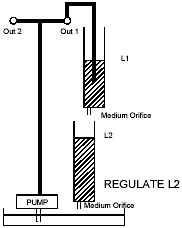
\includegraphics{images/1_relatorio/config_2.png}
    \caption{Sistema de tanques Acoplados}
    \label{fig:sistema_de_tanques_acoplados}
\end{figure}

\newpage
 \cite{scilab2010}   
 
 
% tem que explicar o que é  sistema dinâmico de tanques acoplados: explicado (copiado do roteiro)
% software SCILAB/Xcos explicado

\end{flushleft}

\newpage

%%%%%%%%%% REFERENCIAL TEÓRICO %%%%%%%

\thispagestyle{main}

\section{REFERENCIAL TEÓRICO}

\subsection{Controladores do tipo PID}\hspace{4ex}

\subsection{Sistemas de Primeira Ordem}\hspace{4ex}

\subsection{Sistemas de Segunda Ordem}\hspace{4ex}


\subsection{Sistemas de Segurança Instrumentados ou Intertravamentos}\hspace{4ex}

\newpage


copiar do roteiro

%%%%%%%%%% METODOLOGIA %%%%%%%%%%%%%%%

\thispagestyle{main}

\section{METODOLOGIA}\hspace{4ex}
de fato escrever alguma coisa, como foi feita a simulação
\newpage

%%%%%%%%%% RESULTADOS %%%%%%%%%%%%%%%

\thispagestyle{main}

\section{RESULTADOS e DISCUSSÕES}\hspace{4ex}
resultados obtidos do simulador e discutir eles
explicar como essa seção foi dividida

\subsection{Controlador P}\hspace{4ex}

\subsection{Controlador PI}\hspace{4ex}

\subsection{Controlador PD}\hspace{4ex}

\subsection{Controlador PID}\hspace{4ex}

\subsection{Controlador PID com filtro na ação derivativa}\hspace{4ex}

\subsection{Controlador PID com filtro anti-reset-windup}\hspace{4ex}

\subsection{Sistema de Controle Mestre-Escravo}

\subsubsection{Controlador Mestre P}

\subsubsection{Controlador Mestre PI}

\subsubsection{Controlador Mestre PD}

\subsubsection{Controlador Mestre PID}

\subsubsection{Controlador Mestre PID com filtro na ação derivativa }

\newpage

%%%%%%%%%% CONCLUSÃO %%%%%%%%%%%%%%%

\thispagestyle{main}

\section{CONCLUSÃO}\hspace{4ex}
O que podemos de fato concluir

\newpage

%%%%%%%% REFERÊNCIAS %%%%%%%%%%%%%%%%%

% \section{REFERÊNCIAS BIBLIOGRÁFICAS}

\bibliographystyle{bib/ppgee}
% Referências bibliográficas (geradas automaticamente)
\phantomsection
\addcontentsline{toc}{section}{Referências}
\bibliography{bib/bibliografia}

\appendix

%Apêndice A
\include{apendice}

\end{document}